% siminos/talks/DDaysE12/DDaysE12.tex      pdflatex DDaysE12
% $Author: predrag $
% $Date: 2012-08-08 16:16:55 +0200 (Wed, 08 Aug 2012) $


% Evangelos Dynamics Days Europe 2012 talk  2012.09.06
% used as template:
% Predrag GT math colloquium                2012.03.26
% derived from
% talks/predrag/continuous/continuous.tex   2011.09.09
% Predrag beamer format                     2011.06.17
% Predrag                                   2011.04.12
% derived from
% siminos/talks/Dresden10/symmReduc.tex 	2010.06.29
% Predrag Eckmann's haeberli slide style    2005.05.03
%    ChaosBook/version 11 slides
%	 from ChaosBook continuous.tex

% might want to use text from
%    predrag/lectures/Goth11/Cphg11abstr.txt
%    predrag/lectures/maribor/11/abscvitancourse.tex

\input ../../inputs/layoutBeamerES
\input ../../inputs/def % no edits, always from dasbuch/book/inputs
\input ../../inputs/defsBeamer
                          \date{{\scriptsize
Dynamics Days Europe\\
 6 September 2012
                          }}

\title{Continuous symmetry reduction\\ in high-dimensional flows
with the method of slices
     }
\author{\underline{Evangelos Siminos}\\
    Max Planck Inst. for the Physics of Complex Systems\vspace{20pt}\\
    Predrag~Cvitanovi\'c \\
    Georgia Tech
}


\begin{document}

\section{Symmetries}

\begin{frame}{}
  \titlepage
\end{frame}

\begin{frame}{Motivation}
 \begin{center}
  \includegraphics[width=0.3\textwidth,clip=true] %,height=0.5\textheight
  {CLEx1x2z}
  ~~~~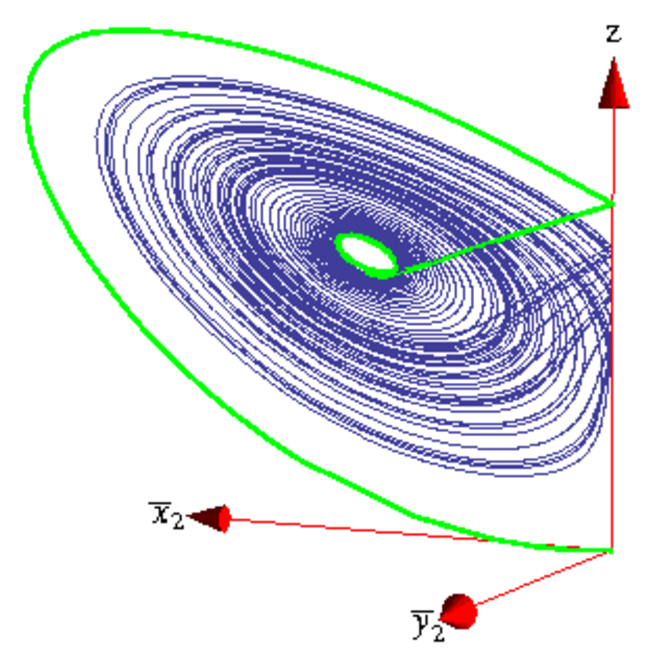
\includegraphics[width=0.3\textwidth,clip=true]
  {CLEinvXYZ}
\end{center}
 \begin{itemize}
  \item Continuous symmetry induces drifts
  \item Transform to equivalent attractor (no loss of information)
  \item ODEs (Complex Lorenz equations)
  \item PDEs (Kuramoto-Sivashinsky equation)
 \end{itemize}

\end{frame}

\begin{frame}{Complex Lorenz equations (CLe)}
 \begin{block}{}
  
 \end{block}

 \begin{block}{Symmetry}
  
 \end{block}


\end{frame}

\begin{frame}{Symmetries of differential equations}
 
\end{frame}

\begin{frame}{CLe solutions}
 
\end{frame}

\begin{frame}{Group orbits}
 
\end{frame}

\section{Symmetry reduction}

\begin{frame}{Symmetry reduction}
 
\end{frame}

\begin{frame}{The method of slices}
 
\end{frame}

\begin{frame}{Application in CLe}
 
\end{frame}

\section{PDEs}

\begin{frame}{Kuramoto-Sivashinsky equation (KSe)}
 
\end{frame}

\begin{frame}{Symmetries of KSe}
 
\end{frame}

\begin{frame}{Solutions of KSe}
 
\end{frame}

\begin{frame}{40000 relative periodic orbits}
 how are they organized?
\end{frame}

\begin{frame}{Relative periodic orbits on a slice}
 
\end{frame}

\begin{frame}{Poincar\'e Section}
 
(No return map) Unstable manifold of shortest orbit organizes the longer orbits

\end{frame}

\begin{frame}{Conclusions and work in progress}
 
 
\end{frame}




\end{document}
